\documentclass{article}

\def\ParSkip{} 
% Packages
\usepackage{amssymb,amsmath,amsthm,bbm}
\usepackage{verbatim,float,url,dsfont}
\usepackage{graphicx,subfigure,psfrag}
\usepackage{algorithm,algorithmic}
\usepackage{mathtools,enumitem}
\usepackage{multirow}
\usepackage{ragged2e}
\usepackage{xr-hyper}
\usepackage{array}

\usepackage[colorlinks=true,citecolor=blue,urlcolor=blue,linkcolor=blue]{hyperref}
\usepackage[margin=1in]{geometry}
\usepackage[round]{natbib}

\usepackage[utf8]{inputenc} % allow utf-8 input
\usepackage[T1]{fontenc}    % use 8-bit T1 fonts
\usepackage{booktabs}       % professional-quality tables
\usepackage{nicefrac}         % compact symbols for 1/2, etc.
\usepackage{microtype}      % microtypography

\ifdefined\TimesFont 
\usepackage{times} % use times font
\fi

\ifdefined\ParSkip 
\usepackage{parskip} % use par skip
\fi

% Theorems and such
\newtheorem{theorem}{Theorem}
\newtheorem{lemma}{Lemma}
\newtheorem{corollary}{Corollary}
\newtheorem{proposition}{Proposition}
\theoremstyle{definition}
\newtheorem{remark}{Remark}
\newtheorem{definition}{Definition}

% Assumption
\newtheorem*{assumption*}{\assumptionnumber}
\providecommand{\assumptionnumber}{}
\makeatletter
\newenvironment{assumption}[2]{
  \renewcommand{\assumptionnumber}{Assumption #1#2}
  \begin{assumption*}
  \protected@edef\@currentlabel{#1#2}}
{\end{assumption*}}
\makeatother

% Widebar
\makeatletter
\newcommand*\rel@kern[1]{\kern#1\dimexpr\macc@kerna}
\newcommand*\widebar[1]{%
  \begingroup
  \def\mathaccent##1##2{%
    \rel@kern{0.8}%
    \overline{\rel@kern{-0.8}\macc@nucleus\rel@kern{0.2}}%
    \rel@kern{-0.2}%
  }%
  \macc@depth\@ne
  \let\math@bgroup\@empty \let\math@egroup\macc@set@skewchar
  \mathsurround\z@ \frozen@everymath{\mathgroup\macc@group\relax}%
  \macc@set@skewchar\relax
  \let\mathaccentV\macc@nested@a
  \macc@nested@a\relax111{#1}%
  \endgroup
}
\makeatother

% Min and max 
\DeclareMathOperator*{\argmin}{argmin}
\DeclareMathOperator*{\argmax}{argmax}
\DeclareMathOperator*{\minimize}{minimize}
\DeclareMathOperator*{\maximize}{maximize}
\DeclareMathOperator*{\find}{find}
\DeclareMathOperator{\st}{subject\,\,to}

% Other operators
\DeclareMathOperator{\Cov}{Cov}
\DeclareMathOperator{\Var}{Var}
\DeclareMathOperator{\dm}{dim}
\DeclareMathOperator{\col}{col}
\DeclareMathOperator{\row}{row}
\DeclareMathOperator{\nul}{null}
\DeclareMathOperator{\rank}{rank}
\DeclareMathOperator{\nuli}{nullity}
\DeclareMathOperator{\spa}{span}
\DeclareMathOperator{\sign}{sign}
\DeclareMathOperator{\supp}{supp}
\DeclareMathOperator{\diag}{diag}
\DeclareMathOperator{\aff}{aff}
\DeclareMathOperator{\conv}{conv}
\DeclareMathOperator{\dom}{dom}
\DeclareMathOperator{\tr}{tr}
\DeclareMathOperator{\df}{df}

% Other shortcuts 
\def\R{\mathbb{R}}
\def\C{\mathbb{C}}
\def\E{\mathbb{E}}
\def\P{\mathbb{P}}
\def\T{\mathsf{T}}
\def\half{\frac{1}{2}}
\def\df{\mathrm{df}}
\def\hy{\hat{y}}
\def\hf{\hat{f}}
\def\hmu{\hat{\mu}}
\def\halpha{\hat{\alpha}}
\def\hbeta{\hat{\beta}}
\def\htheta{\hat{\theta}}
\def\indep{\perp\!\!\!\perp}
\def\th{^{\textnormal{th}}}

\def\cA{\mathcal{A}}
\def\cB{\mathcal{B}}
\def\cD{\mathcal{D}}
\def\cE{\mathcal{E}}
\def\cF{\mathcal{F}}
\def\cG{\mathcal{G}}
\def\cK{\mathcal{K}}
\def\cH{\mathcal{H}}
\def\cI{\mathcal{I}}
\def\cL{\mathcal{L}}
\def\cM{\mathcal{M}}
\def\cN{\mathcal{N}}
\def\cP{\mathcal{P}}
\def\cS{\mathcal{S}}
\def\cT{\mathcal{T}}
\def\cW{\mathcal{W}}
\def\cX{\mathcal{X}}
\def\cY{\mathcal{Y}}
\def\cZ{\mathcal{Z}}


\title{Lecture 7: Exponential Smoothing with Trend and Seasonality \\ 
\Large And a Brief Tour of Other Popular Forecasting Methods \\ \smallskip
\large Introduction to Time Series, Fall 2023 \\ \smallskip
Ryan Tibshirani}
\date{}

\begin{document}
\maketitle
\RaggedRight
\vspace{-50pt}

Related reading: Chapters 8, 9.10, 12.2, and 12.4 of Hyndman and Athanasopoulos
(HA).

\section{Simple exponential smoothing}

\begin{itemize}
\item Exponential smoothing is arguably the other---outside of ARIMA---most 
  popular basic framework for forecasting in time series. These two frameworks
  bear a neat connection, which you saw at the end of the last lecture on ARIMA,
  and which we'll revisit a bit later in this lecture

\item We'll begin with the simplest possible exponential smoother, called
  (unsurprisingly?) \emph{simple exponential smoothing} (SES). This constructs 
  a 1-step ahead forecast via
  \begin{equation}
  \label{eq:ses}
  \hat{x}_{t+1 | t }= \alpha x_t + (1-\alpha) \hat{x}_{t | t-1}
  \end{equation}
  where $\alpha \in [0,1]$ is a parameter to be estimated

\item In other words, the SES forecast \eqref{eq:ses} is a weighted combination 
  of the current observation $x_t$ and the previous forecast \smash{$\hat{x}_{t
      | t-1}$} 

\item By unraveling the iteration, which is basically the same calculation that
  we did in the ARIMA lecture (but now in the opposite direction), this can also
  be written as    
  \begin{equation}
  \label{eq:ses-exp}
  \hat{x}_{t+1 | t} = \alpha x_t + \alpha (1-\alpha) x_{t-1} + \alpha
  (1-\alpha)^2 x_{t-2} + \dots
  \end{equation}
  This explains its name, since observations $x_{t-k}$ that are $k$ steps into 
  the past are exponentially-downweighted, with weight $(1-\alpha)^k$  

\item  (Note: we are being intentionally vague here about the boundary 
  condition. In ARIMA, to develop the theory cleanly, we let time extend back to
  $-\infty$. In  exponential smoothing, we instead usually index time starting
  at $t = 0$, in which case the right-hand side in \eqref{eq:ses-exp} would end
  with $\alpha (1-\alpha)^t x_0$)

\item To make $h$-step ahead forecasts, we iterate \eqref{eq:ses}, where (as 
  usual) we replace future observations by their forecasts. This simply  
  yields \smash{$\hat{x}_{t+2 | t} = \alpha \hat{x}_{t+1 | t} + (1-\alpha)
    \hat{x}_{t+1 | t} = \hat{x}_{t+1 | t}$}, and in general, 
  \begin{equation}
  \label{eq:ses-h}
  \hat{x}_{t+h | t} = \alpha x_t + (1-\alpha) \hat{x}_{t | t-1}
  \end{equation}
  for all horizons $h \geq 1$. That is, SES generates \emph{flat} forecast
  trajectories. We'll see how to extend this to accomodate a trend, shortly  

\item While SES smoothing is already very intuitive, we can motivate it in
  different way, as follows. The \emph{naive flatline forecaster} produces
  forecasts via
  \begin{equation}
  \label{eq:flatline-h}
  \hat{x}_{t+h | t} = x_t 
  \end{equation}
  i.e., it just propogates the last observation forward. Meanwhile, the
  \emph{naive average forecaster} produces forecasts via
  \begin{equation}
  \label{eq:average-h}
  \hat{x}_{t+h | t} = \frac{1}{t} \sum_{i=1}^t x_i
  \end{equation}
  Often we want something in between these two extremes, and that something is  
  given to us by exponential smoothing, recalling the form in \eqref{eq:ses-exp} 
\end{itemize}

\subsection{Component form}

\begin{itemize}
\item For the developments that follow, it is helpful to rewrite the SES forecast
  \eqref{eq:ses-h} in what is known as \emph{component form}

\item Specifically, we think of a ``hidden'' level $\ell_t$ that we are tracking
  over time, that base our forecasts on:
  \begin{equation}
  \label{eq:ses-component}
  \begin{aligned}
  \hat{x}_{t+h | t} &= \ell_t \\
  \ell_t &= \alpha x_t + (1-\alpha) \ell_{t-1}
  \end{aligned}
  \end{equation}

\item The representation in \eqref{eq:ses-component} may appear as kind of a
  trivial rewriting of \eqref{eq:ses-h}, where we replace \smash{$\hat{x}_{t+1 |
      t}$} by $\ell_t$, and \smash{$\hat{x}_{t | t-1}$} by $\ell_{t-1}$. 
  Nonetheless, it serve as a useful jumping off point to extend the model in the 
  next section   

\item Before moving on, we give a brief example of SES from HA, to forecast
  internet useage per minute. The data and SES forecast are shown in Figure
  \ref{fig:internet}, top row. In order to carry out the forecast, we have to
  estimate the smoothing parameter $\alpha$ in \eqref{eq:ses-component}. This is 
  typically done by maximum likelihood (more later), and is what is implemented
  as the default in the \verb|ETS()| function in the \verb|fable| package 

\begin{figure}[p]
\centering
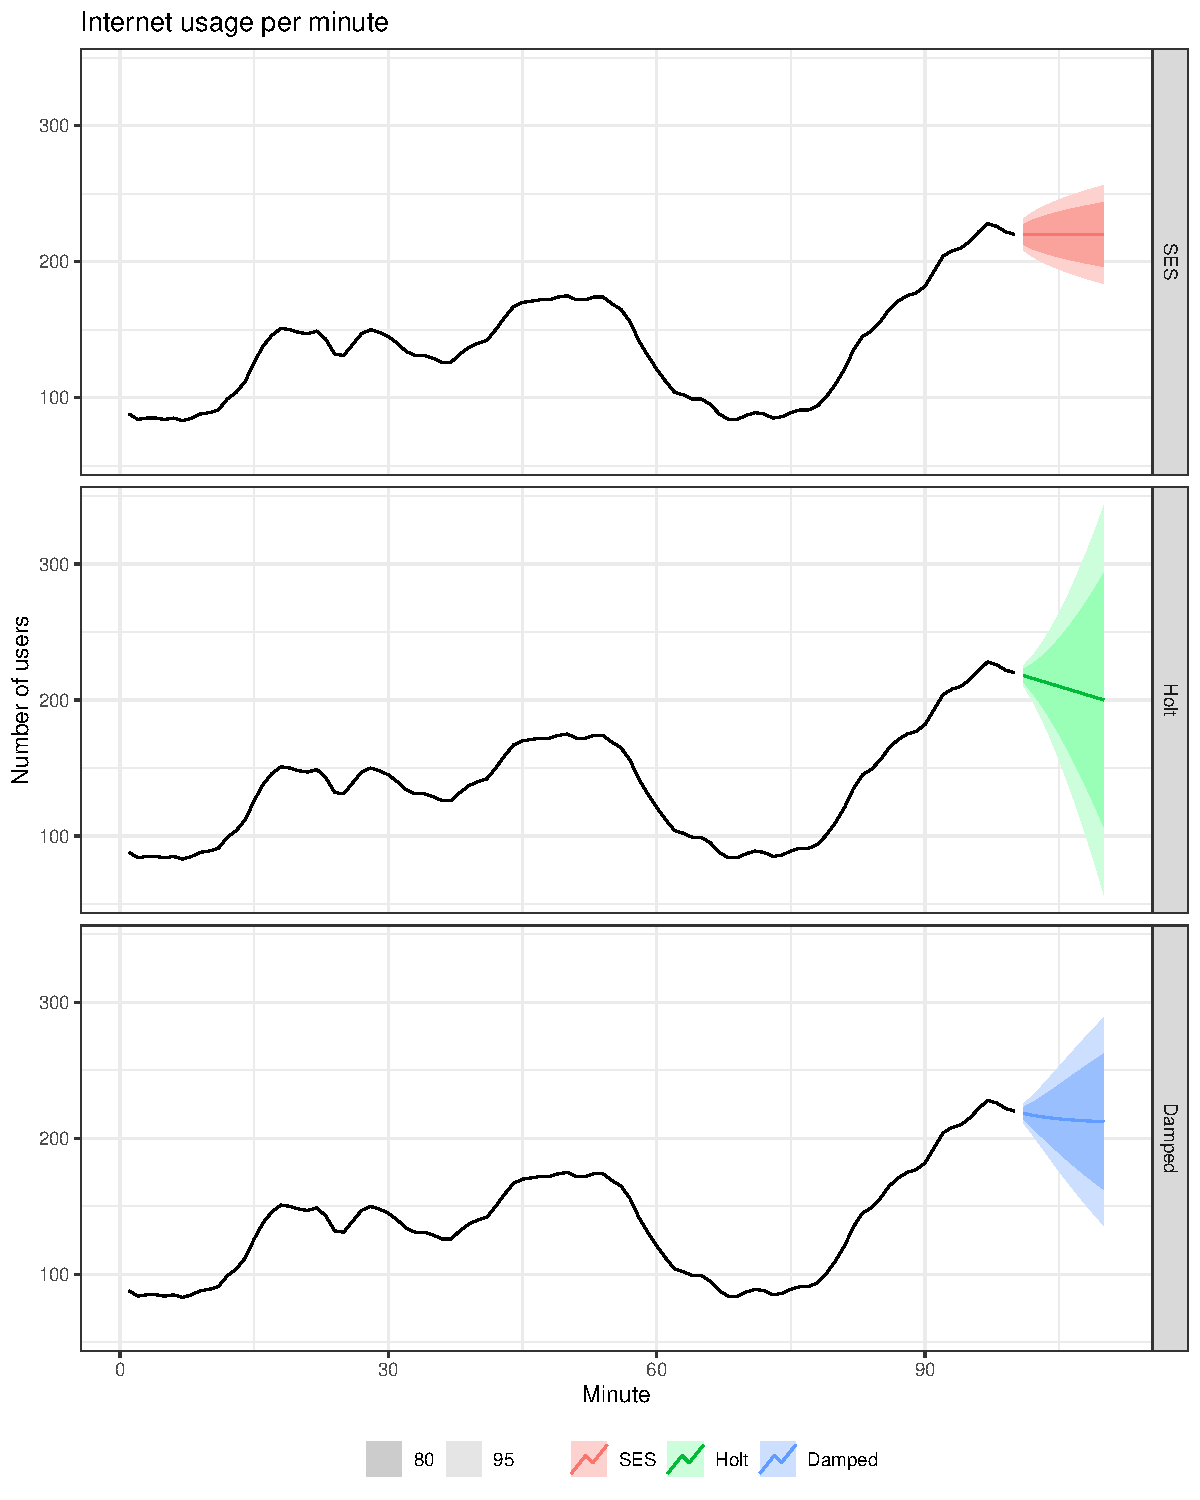
\includegraphics[width=0.95\textwidth]{fig/internet-1.pdf}
\caption{Forecasts on internet useage data (from HA) at 10-steps ahead, from
  three different exponential smoothing models: simple exponential smoothing
  (top), Holt's linear trend (middle), and damped linear trend (bottom).}  
\label{fig:internet}
\end{figure}

\item The forecast from SES is not very impressive, and honestly, in general,
  SES should probably only be viewed as a small step up from the naive
  forecasters \eqref{eq:flatline-h}, \eqref{eq:average-h} 

\item The forecast trajectory from SES is flat, by construction (as previously
  noted). Next we'll see how to extend the method to accommodate a linear trend  
\end{itemize}

\section{Trend extensions}

\begin{itemize}
\item An extension of the SES forecaster in \eqref{eq:ses-component} is
  \emph{Holt's linear trend} method. This changes both the forecast equation
  (first line) and the level equation (second line) to accomodate an estimate of
  the slope $b_t$ of the series at time $t$. We add a trend equation to evolve
  the slope component 

\item Precisely, Holt's linear trend method in component form (which we will
  stick to henceforth) is:
  \begin{equation}
  \label{eq:holt}
  \begin{aligned}
  \hat{x}_{t+h | t} &= \ell_t + b_t h \\
  \ell_t &= \alpha x_t + (1-\alpha) (\ell_{t-1} + b_{t-1}) \\
  b_t &= \beta (\ell_t - \ell_{t-1}) + (1-\beta) b_{t-1} 
  \end{aligned}
  \end{equation}
  Now $\beta$ is an additional parameter to be estimated, where both $\alpha,
  \beta \in [0,1]$ 

\item As before, the level equation updates $\ell_t$ as an $\alpha$-weighted
  combination of the current observation $x_t$ and the previous 1-step ahead
  forecast \smash{$\hat{x}_{t | t-1} = \ell_{t-1} + b_{t-1}$} 

\item The trend equation updates $b_t$ as a $\beta$-weighted combination of the
  current trend $\ell_t - \ell_{t-1}$ and the previous trend $b_{t-1}$

\item Critically, the forecast trajectory from Holt's linear trend method is no
  longer flat but (as the name suggests, and as is apparent from
  \eqref{eq:holt}) a linear function, with slope $b_t$

\item The middle row of Figure \ref{fig:internet} shows the forecast from Holt's
  linear trend method on the internet useage today. To be clear, now both
  $\alpha,\beta$ have been estimated from the data. We can see that it predicts
  a downward trajectory, since $b_t$ at the last time $t$ appears to be
  negative. However, its prediction intervals are very wide, suggesting that the 
  model is highly uncertain of trend directionality  
\end{itemize}

\subsection{Damped trends}

\begin{itemize}
\item Linear trend forecasts at long horizons can be somewhat erratic; we've 
  already seen that the forecast variance is quite high in the example in Figure
  \ref{fig:internet} (as evidenced by the wide prediction intervals) and this
  wasn't even a super long horizon ...

\item As a kind of regularization, we can \emph{dampen} the forecasts from
  Holt's linear trend method. This is often called \emph{damped Holt's} or the
  \emph{damped linear trend} method 

\item In addition to $\alpha,\beta \in [0,1]$ as in \eqref{eq:holt}, we
  introduce a third parameter $\phi \in [0,1]$, to dampen the forecast
  trajectory: 
  \begin{equation}
  \label{eq:damped}
  \begin{aligned}
  \hat{x}_{t+h | t} &= \ell_t + b_t (\phi + \phi^2 + \cdots + \phi^h) \\ 
  \ell_t &= \alpha x_t + (1-\alpha) (\ell_{t-1} + b_{t-1} \phi) \\
  b_t &= \beta (\ell_t - \ell_{t-1}) + (1-\beta) b_{t-1} \phi
  \end{aligned}
  \end{equation}
  Note that when $\phi = 1$, this reduces to Holt's linear trend method in
  \eqref{eq:holt} 

\item The interpretation in the damped method \eqref{eq:damped} is mostly the
  same as in Holt's method \eqref{eq:holt}, but you can think of the
  modification like this: the contribution of a given slope to a forecast in the
  future diminishes at each step into the future, by a multiplicative factor of
  $\phi$   

\item As $h \to \infty$, the forecasts from the damped linear trend method
  approach a particular constant (finite) level, namely
  \[
  \hat{x}_{t+h | t} \to \ell_t + b_t \sum_{j=1}^\infty \phi^j = \ell_t + b_t
  \frac{\phi}{1-\phi} 
  \]
  For example, when $\phi = 0.9$, this limit is $\ell_t + 9 b_t$

\item HA say that a practical range for $\phi$ is usually 0.8 to 0.98; when
  $\phi$ is below 0.8, the dampening is too strong (and short-term forecasts are
  not ``trended'' enough); when $\phi$ is above 0.98, it is too weak (and you
  cannot distinguish the forecasts from Holt's linear trend method for
  reasonably horizons). In fact, the \verb|ETS()| function limits the range of
  $\phi$ to be $[0.8, 0.98]$, by default

\item The bottom row of Figure \ref{fig:internet} shows the forecasts from the
  damped linear trend method on the internet useage data. To be clear, all of 
  $\alpha,\beta,\phi$ are estimated from the data. We can see a weak downward
  trend, that is quickly attenuated. The prediction intervals are also much 
  narrower. Inspection of the fitted model (see the R notebook) shows that we
  the dampening coeffcient estimate is \smash{$\hat\phi = 0.81$}, so it has
  quite a pronounced effect here
\end{itemize}

\section{Seasonality extensions}

\begin{itemize}
\item To account for seasonality, on top of trend, we can use what is called the   
  \emph{Holt-Winters} method. This changes the forecast and level equations in
  \eqref{eq:holt} in order to adjust for a seasonal effect, but the trend
  equation stays the same. We add a seasonality equation to evolve the seasonal
  component    

\item We assume a known seasonal period $m$. That is, observations occurring
  every $m$ time points share a common (but unknown) seasonal effect. The
  Holt-Winters method is then:  
  \begin{equation}
  \label{eq:holt-winters}
  \begin{aligned}
  \hat{x}_{t+h | t} &= \ell_t + b_t h + s_{t+h-mk} \\  
  \ell_t &= \alpha (x_t - s_t) + (1-\alpha) (\ell_{t-1} + b_{t-1}) \\ 
  b_t &= \beta (\ell_t - \ell_{t-1}) + (1-\beta) b_{t-1} \\
  s_t &= \gamma (x_t - \ell_t) + (1-\gamma) s_{t-m}
  \end{aligned}
  \end{equation}
  The parameters of the model are $\alpha,\beta,\gamma \in [0,1]$

\item In the forecast equation (first line), we define $k \geq 0$ to be the
  integer such that $t+h-mk \in [t-m, t]$: the seasonal component we are using
  to adjust the forecast should be the latest one (whatever was available in the
  last period). This is equivalent to seeking $mk \in [h, h+m]$. You can check
  that this is accomplished by setting \smash{$k = \lceil h/m \rceil$} 

\item The interpretation of Holt-Winters \eqref{eq:holt-winters} is similar to 
  Holt's method \eqref{eq:holt}, except that we \emph{seasonally-adjust} the 
  observations in the level and trend equations. The seasonal equation updates
  $s_t$ as a $\gamma$-weighted combination of the level-adjusted observation
  $x_t - \ell_t$ and the previously-relevant seasonal component $s_{t-m}$   

\item (We can also introduce dampening into \eqref{eq:holt-winters}, which is
  just as in \eqref{eq:damped}, but we skip writing this out for brevity)

\item Figure \ref{fig:} shows an example of Holt-Winters in action, on
  Australian holiday travel data from HA. Its ability to pick up (and evolve!)
  seasonality is impressive. This is arguably the most powerful aspect of
  exponential smoothing methods in general (more so than their ability to model
  and evolve trends)  


\end{itemize}

\subsection{Multiplicative version}

\begin{itemize}
\item 
\item A multiplicative version of tracking trends is also possible. HA  
\end{itemize}

\section{ETS models}

\begin{itemize}
\item Multiplicative errors and trends
\item HA do not recommend multiplicative trend?
\end{itemize}

\subsection{State space representation}

\begin{itemize}
\item 
\end{itemize}

\subsection{Estimation and selection}

\begin{itemize}
\item 
\end{itemize}

\subsection{Forecasting}

\begin{itemize}
\item 
\end{itemize}

\subsection{ARIMA versus ETS}
\begin{itemize}
\item 
\end{itemize}

\section{Theta model}

\section{Prophet model}

\section{Neural network AR}



\end{document}
